\documentclass[11pt]{article}
\usepackage[a4paper,margin=0.82in]{geometry}
\usepackage[T1]{fontenc}
\usepackage{newtxtext,newtxmath,microtype,booktabs,array,tabularx,siunitx,xcolor,tikz,amsmath,enumitem,float,fancyhdr,hyperref,graphicx}
\usepackage[nameinlink,noabbrev]{cleveref}
\usetikzlibrary{arrows.meta,positioning}
\definecolor{MisulInk}{HTML}{171E2B}
\definecolor{MisulBlue}{HTML}{0866C6}
\definecolor{MisulGray}{HTML}{687386}
\definecolor{RuleGray}{HTML}{D7DCE2}
\definecolor{PanelGray}{HTML}{F5F7FA}
\newcommand{\misulmark}[1]{%
  \begin{tikzpicture}[x=#1cm,y=#1cm,baseline=0.2ex]
    \fill[MisulInk]
      (5,0) -- (5,12) arc (180:0:6) arc (180:0:6)
      -- (29,0) -- (22,0) -- (22,9) arc (0:180:2.5)
      -- (17,0) -- (12,0) -- (12,12) arc (0:180:1)
      -- (10,0) -- cycle;
  \end{tikzpicture}%
}
\newcommand{\misulfooter}{\misulmark{0.016}\hspace{0.38em}\footnotesize Misul}
\hypersetup{colorlinks=true,linkcolor=MisulBlue,citecolor=MisulBlue,urlcolor=MisulBlue,
pdftitle={Interlace: A Shared Architecture for Language and Iterative Computation},pdfauthor={Deyan Todorov}}
\pagestyle{fancy}
\fancyhf{}
\fancyhead[L]{\small Misul | Architecture and system card}
\fancyhead[R]{\small Misul}
\fancyfoot[L]{\misulfooter}
\fancyfoot[R]{\footnotesize\thepage}
\renewcommand{\headrulewidth}{0.35pt}
\renewcommand{\footrulewidth}{0pt}
\setlength{\headheight}{14pt}
\setlength{\parindent}{1em}
\setlength{\parskip}{0.2em}
\setlist{nosep,leftmargin=*}
\sisetup{detect-all,group-separator={,},group-minimum-digits=4}
\newcommand{\code}[1]{\texttt{#1}}
% Generated from the verified complete precision pair; do not edit numbers by hand.
\newcommand{\MisulValidationDelta}{+0.49}
\newcommand{\MisulTestDelta}{+0.56}
\newcommand{\MisulReleaseBytes}{31026301}
\newcommand{\MisulStandardFlow}{10.94}
\newcommand{\MisulStandardValDelta}{+3.75}
\newcommand{\MisulStandardMinutes}{5.36}
\newcommand{\MisulFixedFlow}{12.50}
\newcommand{\MisulFixedValDelta}{+3.75}
\newcommand{\MisulFixedMinutes}{6.67}
\newcommand{\MisulFPValidation}{4.7419}
\newcommand{\MisulFPTest}{4.7602}
\newcommand{\MisulFPBitsPerByte}{1.9619}
\newcommand{\MisulFPMinutes}{58.77}
\newcommand{\MisulFPPhysicalGB}{1.239}
\newcommand{\MisulFPStreamHeld}{100.00}
\newcommand{\MisulFPStreamLong}{92.97}
\newcommand{\MisulFPIdleThought}{9.77}
\newcommand{\MisulFPFlowLong}{0.00}
\newcommand{\MisulFPFlowNoFeedback}{0.00}
\newcommand{\MisulFPFlowOne}{0.39}
\newcommand{\MisulFPFlowTwo}{1.56}
\newcommand{\MisulFPFlowFour}{1.56}
\newcommand{\MisulFPFlowEight}{1.95}
\newcommand{\MisulFPRetries}{3}
\newcommand{\MisulBFValidation}{4.7187}
\newcommand{\MisulBFTest}{4.7339}
\newcommand{\MisulBFBitsPerByte}{1.9511}
\newcommand{\MisulBFMinutes}{22.03}
\newcommand{\MisulBFPhysicalGB}{1.109}
\newcommand{\MisulBFStreamHeld}{100.00}
\newcommand{\MisulBFStreamLong}{80.47}
\newcommand{\MisulBFIdleThought}{9.38}
\newcommand{\MisulBFFlowLong}{0.00}
\newcommand{\MisulBFFlowNoFeedback}{0.00}
\newcommand{\MisulBFFlowOne}{0.00}
\newcommand{\MisulBFFlowTwo}{0.00}
\newcommand{\MisulBFFlowFour}{0.00}
\newcommand{\MisulBFFlowEight}{0.00}
\newcommand{\MisulBFRetries}{12}
\newif\ifmisulprecisionpassed
\misulprecisionpassedtrue
\newif\ifmisulfixedpointpassed
\misulfixedpointpassedfalse


\newcommand{\ModelName}{Interlace}
% Generated from verified architecture evidence.
\newcommand{\DenseValidation}{5.2278}
\newcommand{\DenseTest}{5.2516}
\newcommand{\DenseBitsPerByte}{2.1645}
\newcommand{\DenseStreamHeld}{100.00}
\newcommand{\DenseStreamLong}{4.69}
\newcommand{\DenseFlowEight}{0.39}
\newcommand{\DenseMinutes}{22.26}
\newcommand{\MisulArchitectureAbstract}{The combined model has 9.86\% lower official test loss at the same training budget. It reaches the fixed 5.5-nat validation-monitor target in 276.52 seconds versus 806.91 seconds for the dense control. Longer-program stream accuracy is 80.47\% versus 4.69\% for the dense control.}
\newcommand{\MisulArchitectureVerdict}{At this fixed budget, the combined model has 9.86\% lower official language-test loss. Total training execution is 1.04\% shorter; this cost includes the disclosed interrupted work. On longer programs, its stream answer accuracy is 80.47\% versus 4.69\%. These are observed differences between the two trained models, not evidence that every architectural component improves performance. Additional seeds, component ablations and independently tuned dense controls remain necessary.}


\begin{document}
\begin{center}
  \misulmark{0.075}\par
  \vspace{0.55em}
  {\LARGE\bfseries \ModelName: A Shared Architecture\par for Language and Iterative Computation\par}
  \vspace{0.7em}
  {\large Deyan Todorov\par}
  \vspace{0.18em}
  {\normalsize Misul\par}
  \vspace{0.25em}
  {\small Research paper and system card\quad |\quad 9 September 2026\par}
\end{center}
\vspace{0.65em}

\noindent\textbf{Abstract.}
\ModelName{} is a shared language architecture designed to improve learned
capability per stored parameter and training budget. It combines bounded
rational features, content-selected attention, gated delta memory and repeated
shared depth. A \num{29814640}-parameter model trained from random initialization
is compared with a \num{29921280}-parameter dense Transformer under the same
BF16 joint training recipe. \MisulArchitectureAbstract{}
These measurements motivate testing whether the architecture can reduce the
cost of reaching useful model quality. Both models use the same synchronous
stream interface; the comparison measures the combined backbone rather than
any isolated component. Results cover one seed, WikiText-2 and bounded
prefix-addition programs. The released FP8 checkpoint provides a compact
reference implementation; Flow-style refinement is an experimental extension.
We specify a staged validation program to test repeatability, component
contributions and transfer to larger data and task budgets.

\section{Introduction}
A model can increase its effective computation without storing a separate
parameter set for every computational stage. It can also combine selective
access to past representations with a recurrent memory that accumulates
information over time. The research question is whether these mechanisms,
trained together, produce more useful capability at a given model size and
training cost.

\ModelName{} integrates four backbone mechanisms: a bounded rational
feed-forward transformation, content-selected attention, gated delta memory,
and a repeated shared stack. Two additional interfaces expose computation in
different ways: synchronous streams produce intermediate states alongside
external inputs, while Flow refinement revises a complete candidate solution.
These interfaces share the language backbone; no external fact store or
teacher supplies their answers.

The central measurement is time to a fixed language-quality target. We report
that quantity alongside final held-out loss, stored parameters and inference
latency. Repeated seeds and controlled architectural changes are needed to
understand how these quantities depend on the combined mechanisms.

The contribution is the implemented combination, its explicit mathematical
contracts and a controlled evaluation at approximately 30 million parameters.
The paper separates architectural quality, training cost, inference cost and
representation precision. A parameter-matched dense control tests the combined
backbone under a common recipe. It does not isolate the contribution of each
component, which requires further ablations.

\section{Architecture}
The model uses width 640, feed-forward width 1,536, eight heads, a
4,096-token byte-level BPE vocabulary and a 128-row context. Six residual blocks
alternate three attention and three memory blocks. The same stack is applied
twice, giving twelve block evaluations with six stored block parameter sets.
Learned role, mode, position and loop embeddings are included in the total
parameter count. Text uses a tied input/output vocabulary matrix. Structured
refinement adds a ten-category output head.

\begin{figure}[H]
\centering
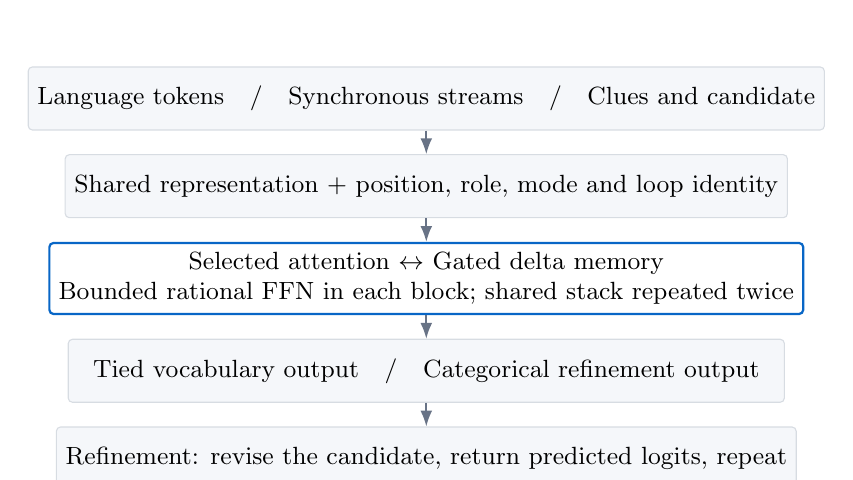
\begin{tikzpicture}[
  node distance=3mm,
  box/.style={draw=RuleGray,fill=PanelGray,rounded corners=1.5pt,minimum height=8mm,minimum width=0.75\textwidth,align=center,font=\small},
  own/.style={box,draw=MisulBlue,thick,fill=white},
  arr/.style={-{Latex[length=2mm]},semithick,draw=MisulGray}]
  \node[box] (input) {Language tokens\quad /\quad Synchronous streams\quad /\quad Clues and candidate};
  \node[box,below=of input] (embed) {Shared representation + position, role, mode and loop identity};
  \node[own,below=of embed] (body) {Selected attention $\leftrightarrow$ Gated delta memory\\Bounded rational FFN in each block; shared stack repeated twice};
  \node[box,below=of body] (heads) {Tied vocabulary output\quad /\quad Categorical refinement output};
  \node[box,below=of heads] (flow) {Refinement: revise the candidate, return predicted logits, repeat};
  \draw[arr] (input)--(embed);\draw[arr] (embed)--(body);\draw[arr] (body)--(heads);\draw[arr] (heads)--(flow);
\end{tikzpicture}
\caption{A common parameter set supports three interfaces. Shared depth repeats
latent computation; refinement explicitly revises predicted candidate states.}
\end{figure}

\subsection{Bounded rational features}
Rational architectures motivate expressive feature interactions beyond a fixed
scalar activation~\cite{cofr,ran}. The feed-forward block uses paired learned
projections and a positive quadratic denominator:
\begin{equation}
 (a,b)=W_{\mathrm{up}}x,\qquad
 r(a,b)=\frac{a(1+b)}{1+a^2+b^2},\qquad
 \operatorname{FFN}(x)=W_{\mathrm{down}}r(a,b).
 \label{eq:gate}
\end{equation}
For fixed $b$, maximizing over $a$ gives
$|r|\le |1+b|/(2\sqrt{1+b^2})\le1/\sqrt2$. The gate therefore bounds the
interaction without a denominator floor. Its derivatives are
\begin{equation}
 \frac{\partial r}{\partial a}=\frac{(1+b)(1+b^2-a^2)}{(1+a^2+b^2)^2},\qquad
 \frac{\partial r}{\partial b}=\frac{a(1+a^2-b^2-2b)}{(1+a^2+b^2)^2}.
\end{equation}
The implementation evaluates an algebraically equivalent scaled expression
using $s=\max(1,|a|,|b|)$ to avoid overflow. The explicit parameterization is
part of this architecture; rational networks themselves have prior art.
A bounded gate alone does not imply greater knowledge capacity.

\subsection{Selected attention and delta memory}
Attention selects two completed eight-row source blocks using content
summaries, together with the current block. Exact softmax attention operates
within the selected mask. This follows the selective-access direction of
Monodratic~\cite{monodratic}; the present implementation does not reproduce its complete index.
Text and stream queries cannot read future rows. Flow can read the full
current candidate because all candidate positions are available at inference.

Memory complements selective reads with a gated delta recurrence~\cite{kda}.
Each head has 16 key coordinates and 80 value coordinates. With normalized
keys and queries and learned decay $\alpha_t$ and write strength $\beta_t$,
\begin{equation}
 \widetilde S_t=\operatorname{diag}(\alpha_t)S_{t-1},\quad
 e_t=v_t-k_t^{\!T}\widetilde S_t,\quad
 S_t=\widetilde S_t+\beta_t k_t e_t,\quad o_t=q_t^{\!T}S_t.
\end{equation}
The memory input is the mean of the current row's role representations. Its
output is gated separately for each role. This state is transient computation;
it is not a persistent retrieval database.

\subsection{Synchronous streams}
The stream interface receives external input digits and predicts thought and
output tokens over successive ticks. The initial task is prefix addition
modulo ten, which provides exact intermediate-state and final-answer labels.
During evaluation, thought and output tokens are generated freely over the
full vocabulary. No reference intermediate state is supplied to inference.

\subsection{Experimental candidate refinement}
The refinement interface adapts Flow Reasoning Models~\cite{frm}. Given clues
$c$, categorical endpoint $y$, Gaussian noise $z$ and time $t$, training uses
$x_t=(1-t)z+ty$. A denoiser predicts category logits
$\ell_\theta(c,x_t,t,f)$, with either zero feedback or detached logits from a
previous prediction. A masked categorical cross-entropy supervises valid
program positions. One quarter of training times are zero, where the
candidate contains no target contribution.

At inference the candidate begins as noise. At each of $K$ uniform steps,
\begin{equation}
 p_i=\operatorname{softmax}(\ell_\theta(c,x_i,t_i,f_i)),\qquad
 x_{i+1}=x_i+\frac{p_i-x_i}{K-i},\qquad f_{i+1}=\ell_\theta(c,x_i,t_i,f_i).
\end{equation}
All candidate positions can change. The evaluated checkpoint uses ordinary
self-conditioning; trajectory-based Fixed-Point Forcing is not part of its
selected training recipe. Re-noise consistency measures stability of a
prediction and must not be interpreted as a correctness certificate.

\section{Experimental method}
\subsection{Data, training and controls}
All models begin from random initialization. The language corpus is
WikiText-2 raw~\cite{wikitext}, with a tokenizer fitted only on its 629 prepared
training documents. Each joint run contains \num{16384} updates:
\num{8192} language updates with \num{4194304} sampled target tokens,
\num{4096} stream updates and \num{4096} Flow updates. Training programs have
lengths two through six. Sequence hashes separate training, validation and test
programs. The fixed final tests contain 256 short and 128 longer programs,
with lengths eight through ten in the latter group.

Hidden matrices use NorMuon updates with five Polar Express iterations,
momentum 0.7, row second moments and update RMS 0.2~\cite{pe,normuon}.
Matrix learning rate is 0.006; embeddings and auxiliary parameters use AdamW
at 0.001. Weight decay is 0.01. The schedule warms up for 64 updates, remains
constant through 80\% of training and decays linearly to one tenth. The
architecture comparison holds the training precision at BF16 and uses the
same seed, batch order, task mixture, optimizer and schedule.

The dense control has six unique full-attention/SwiGLU blocks~\cite{swiglu},
applied once, with width 640 and hidden width 1,504. It retains the same tied
embedding and text/stream/Flow adapters so that task access is comparable.
Its \num{29921280} parameters exceed the combined model by only 0.36\%.
It has no delta-memory blocks, rational gates, content-selected mask or
repeated shared stack. This is a matched comparison of two concrete
architectures under a common recipe, not an independently tuned search over
dense models.

\subsection{Measurement and reproducibility}
Language quality uses all 2,488 official validation and 2,844 official test
windows. The test corpus is assembled from the same pinned source revision;
its documents have no title, whole-document or normalized paragraph overlap
of at least 80 characters with the prepared training and validation data.
The dense recipe is fixed before opening its test results. The baseline is a
new comparison against an already evaluated model, not a blind model-selection
competition.

We report exact sequence and final-answer accuracy separately. Longer inputs
test length generalization beyond training. Disabling generated thought and
removing feedback are inference interventions, not retrained ablations.
Numerical checks compare rational and dense feed-forward values and gradients,
attention masks and memory recurrence against independent host calculations.

Elapsed training cost includes initialization, compilation, data handling,
validation, checkpoint handling, numerical retries and interrupted execution.
The combined BF16 run includes recovery after an overflow; the original failed
run remains in the record. First observed monitor crossings at 6.0, 5.5 and
5.0 nats/token are measured at fixed 512-update intervals, without interpolating
an unobserved crossing. Inference measurements synchronize completed device
work and use eighteen repetitions across two fresh processes per model, in a
counterbalanced order, after separately reported first executions.
Generation uses the same uncached implementation in both arms. Measurements
use one local accelerator and a bounded process working set; hardware,
software versions, raw times, resource records and checksums accompany the
technical supplement. Distributed performance is outside this evaluation.

\section{Results}
\subsection{Architecture comparison}
\begin{table}[H]
\centering
\begin{tabularx}{\textwidth}{@{}Xrr@{}}
\toprule
Measurement & \ModelName{} BF16 & Dense BF16\\
\midrule
Parameters, millions & 29.815 & 29.921\\
Full validation loss, nats/token & \MisulBFValidation & \DenseValidation\\
Official test loss, nats/token & \MisulBFTest & \DenseTest\\
Official test bits/byte & \MisulBFBitsPerByte & \DenseBitsPerByte\\
Held-out stream answers (\%) & \MisulBFStreamHeld & \DenseStreamHeld\\
Longer-program stream answers (\%) & \MisulBFStreamLong & \DenseStreamLong\\
Held-out eight-pass Flow, exact (\%) & \MisulBFFlowEight & \DenseFlowEight\\
Total training execution, minutes & \MisulBFMinutes & \DenseMinutes\\
\bottomrule
\end{tabularx}
\caption{Equal update and language-token budgets, common BF16 precision and
one seed. All task scores come from the same final checkpoint in each arm.}
\end{table}

\MisulArchitectureVerdict{}

\begin{figure}[H]
\centering
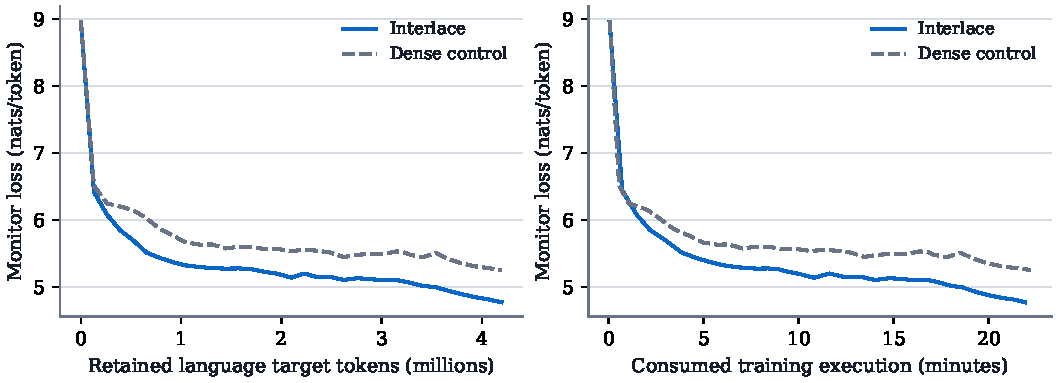
\includegraphics[width=\textwidth]{figures/misul_architecture.pdf}
\caption{Language learning at matched retained token budgets and measured
execution time. Curves use the same fixed 32-window validation monitor;
full-split results are reported in the table. Retried work is included in time.}
\end{figure}

\begin{table}[H]
\centering
\begin{tabularx}{\textwidth}{@{}Xrr@{}}
\toprule
First observed monitor target, seconds & \ModelName{} BF16 & Dense BF16\\
\midrule
6.0 nats/token & 131.29 & 204.37\\
5.5 nats/token & 276.52 & 806.91\\
5.0 nats/token & 1115.28 & Not reached\\
\bottomrule
\end{tabularx}
\caption{Time to a fixed monitor quality, sampled every 512 updates. Each time
includes consumed training execution before the observed crossing.}
\end{table}
\begin{table}[H]
\centering
\begin{tabularx}{\textwidth}{@{}Xrr@{}}
\toprule
Inference latency, median & \ModelName{} BF16 & Dense BF16\\
\midrule
128-token forward, batch 1 (ms) & 6.14 & 2.11\\
Generate 32 tokens, batch 1 (s) & 0.11 & 0.04\\
Eight-pass Flow, batch 8 (ms) & 30.60 & 10.63\\
\bottomrule
\end{tabularx}
\caption{Eighteen completed-device repetitions per workload across two
counterbalanced processes per model, after separately recorded first executions. Both models use BF16 and the same uncached generation
procedure. These are local implementation measurements.}
\end{table}


The dense control has lower latency in all three reported inference workloads.
The measured improvement in held-out quality and earlier monitor crossings
therefore accompanies higher inference latency in this implementation.


\subsection{Reference checkpoint and precision}
The reference checkpoint uses FP8 weights and projection operands, with wider
working tensors. Its complete learned tensor payload, including padding and
scales, is 48.44\% smaller than an equal-parameter BF16 representation; the
weight file is 30.76 MB. Relative language loss differs by
\MisulValidationDelta\% on validation and \MisulTestDelta\% on the official
test against the same architecture trained in BF16. Both are below the
registered 1\% precision threshold for this pair. This is a secondary
representation result, separate from the architectural comparison above.

Free-running streams produce \MisulFPStreamHeld\% correct held-out answers
and \MisulFPStreamLong\% on longer programs. Clamping the thought stream to
idle lowers held-out accuracy to \MisulFPIdleThought\%. These results show a
learned intermediate-state dependency on the evaluated task. Since the dense
control uses the same stream interface, its comparison with Interlace cannot
isolate the stream mechanism as the cause of the accuracy difference.

Eight-pass Flow produces \MisulFPFlowEight\% exact held-out state sequences,
versus \MisulFPFlowOne\% after one pass. It produces no exact longer-program
sequences in this test. The implemented mechanism supports candidate revision,
but reliable refinement remains an open capability gate. Language samples
exhibit repetition and fragmented continuations; no general question-answering
benchmark has been passed.

\section{System card}
\begin{table}[H]
\centering
\small
\begin{tabularx}{\textwidth}{@{}p{0.23\textwidth}X@{}}
\toprule
Field & Current specification\\
\midrule
Developer & Deyan Todorov, Misul\\
Model & Approximately 30M parameters; shared language, stream and refinement backbone\\
Initialization & Random; no pretrained checkpoint, teacher distillation or external answer store\\
Language data & WikiText-2 raw; train-only byte-level BPE, vocabulary 4,096\\
Structured data & Synthetic prefix-sum programs modulo ten; training lengths 2--6\\
Context & Up to 128 rows; one language stream or three synchronous roles\\
Outputs & Autoregressive tokens, generated intermediate/final program tokens, or categorical candidate states\\
Intended use & Architecture research, controlled capability evaluation and reproducible inference experiments\\
Current limits & Fragmented text; weak Flow exact accuracy; no demonstrated general instruction following or factual QA\\
Training state & BF16 working parameters and optimizer; separately counted from the compact released weights\\
Release status & Research checkpoint and reproducibility package; Apache-2.0 license\\
Evaluation scope & One training seed for the 30M dense comparison; fixed short context and bounded synthetic programs\\
\bottomrule
\end{tabularx}
\caption{The system card describes the evaluated checkpoint, rather than an
anticipated larger model.}
\end{table}

The current model has not undergone a comprehensive bias, memorization,
robustness or misuse evaluation. Generated text can be incorrect or reproduce
patterns in the training corpus. The architecture does not implement tool use,
autonomous actions or a persistent external memory. The reproducibility
package preserves failed examples alongside successful outputs and includes
model, tokenizer and source digests.

\section{Validation program}
The next study tests whether the observed learning advantage survives new
seeds, architectural controls and broader workloads. The following are
prospective decision criteria, not additional results. Protocols, data splits,
resource caps and analysis scripts will be frozen before confirmation runs.

\paragraph{Repeatability.}
Run three fresh paired seeds with unchanged recipes. Use paired summaries of
full validation loss and first observed time to the fixed 5.5-nat monitor target;
retain every seed, interruption and failed crossing. Advance if all three pairs
improve full validation loss and median time to target is at least 10\% lower.
If the target is not reached within the common cap, record a non-crossing rather
than extrapolating time. Open the final test only after the recipes are fixed.

\paragraph{Mechanism and baseline.}
Screen rational-gate, attention-selection, delta-memory and shared-depth
ablations under the same data budget, reporting parameter count and actual
execution cost. Add a dense shared-depth control to distinguish depth reuse
from the other changes. Give both architecture families equal validation-only
optimizer-tuning budgets. Confirm promising contrasts with three new paired
seeds. Attribute a component only when its removal worsens validation loss in
all confirmation pairs; interactions remain possible.

\paragraph{Transfer.}
Evaluate the selected recipe on a separate broader corpus, longer contexts and
an additional structured task. Select that task and its success threshold before
training. Require lower validation loss and at least 10\% less median time to a
predeclared quality target across three fresh pairs before advancing the scale
claim. Measure inference latency and total stored state alongside training cost.
A smaller numerical and resource pilot precedes every workload increase.

Training efficiency and inference latency remain separate measurements across
all stages. Refinement proceeds as a separate research extension, with
exact-solution gains across passes required before it becomes a primary
capability claim.

\begin{thebibliography}{9}
\small\raggedright\setlength{\itemsep}{0pt}
\bibitem{cofr} A. Dhurandhar et al. \emph{CoFrGeNet: Continued Fraction Architectures for Language Generation}. 2026. \url{https://arxiv.org/abs/2601.21766}.
\bibitem{ran} J. Zhang et al. \emph{Rational ANOVA Networks}. 2026. \url{https://arxiv.org/abs/2602.04006}.
\bibitem{kda} Kimi Team. \emph{Kimi Linear: An Expressive, Efficient Attention Architecture}. 2025. \url{https://arxiv.org/abs/2510.26692}.
\bibitem{frm} A. Helbling et al. \emph{Flow Reasoning Models: Turning Flows Into Efficient Recurrent Reasoners}. 2026. \url{https://arxiv.org/abs/2606.29150}.
\bibitem{pe} N. Amsel et al. \emph{The Polar Express: Optimal Matrix Sign Methods and Their Application to the Muon Algorithm}. 2025. \url{https://arxiv.org/abs/2505.16932}.
\bibitem{normuon} Z. Li et al. \emph{NorMuon: Making Muon more efficient and scalable}. 2025. \url{https://arxiv.org/abs/2510.05491}.
\bibitem{swiglu} N. Shazeer. \emph{GLU Variants Improve Transformer}. 2020. \url{https://arxiv.org/abs/2002.05202}.
\bibitem{wikitext} Salesforce. \emph{WikiText-2 raw v1}. Pinned revision and data preparation records accompany the reproducibility package. \url{https://huggingface.co/datasets/Salesforce/wikitext}.
\bibitem{monodratic} D. Todorov. \href{https://github.com/MisulOrg/Monodratic/blob/main/output/pdf/monodratic_proof.pdf}{\emph{Monodratic: A Sparse Attention Architecture with Learned Product-Hash Routing}}. Technical report, 2026.
\end{thebibliography}
\end{document}
